\section{Similar Face Recognition Using the IE-CNN Model}

\begin{center}
    \author{
    An-Ping Song,
    Qian Hu,
    Xue-Hai Ding,
    Xin-Yi Di,
    Zi-Heng Song
    }
\end{center}

\begin{center}
    \emph{DIGITAL OBJECT IDENTIFIER}
\end{center}

\subsection{INTRODUCTION}
Currently there are few datasets that provide a set of images with faces of 
similar people, moreover there are few methods tested to be able to verify 
the level of similarity. Two types of work are carried out in the following paper. 
The first is based on proposing a procedure for creating a large dataset of 
similar faces that requires a small amount of man-force to label the content. 
In the second work, instead, an IE-CNN model is built which has the task 
of improving the internal and external features of the face, increasing the 
precision of face matching.

\subsection{RELATED WORK}
Unlike objects that may have a similar shape or color, the human face may 
have similar external (located at head, chin and ears) or internal (eyes, nose 
and mouth) structural features. However, many recognition algorithms tend 
to discard external features and only work with internal ones. To understand 
the importance of using both categories of features, just look at the image \ref{fig:features} 
where there are similar faces (internal features) but different physical structures 
of the skull (external features), or the opposite. The proposed model 
(\emph{IE-CNN}) deals with improving facial features using a CNN network.
\begin{figure}[h!]
    \centering
    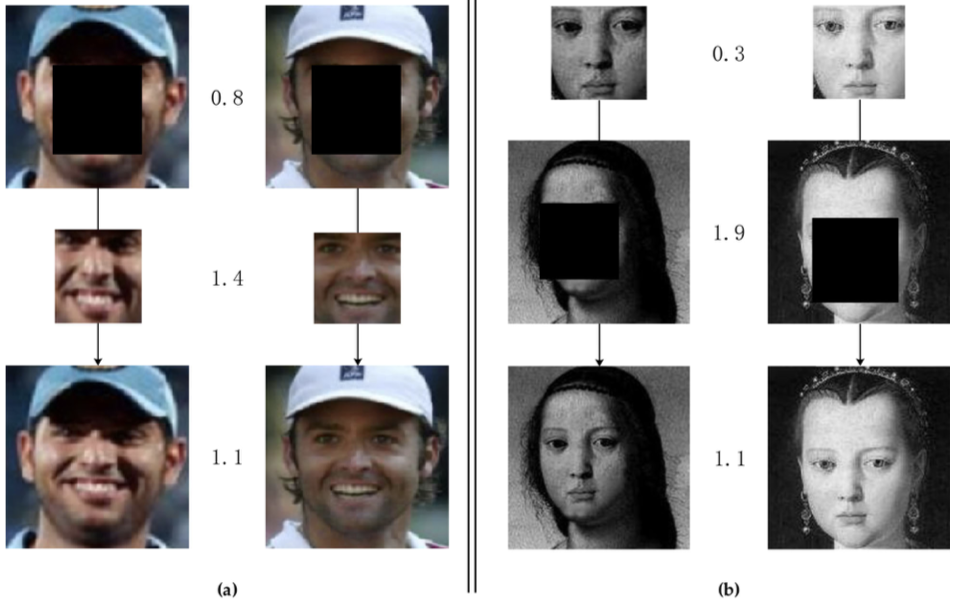
\includegraphics[width = 0.8\linewidth]{images/paper9/importance.png}
    \centering
    \caption{(a) Shows the importance of internal features and (b) shows the importance of external features. The values are the cosine distances.}
    \label{fig:features}
\end{figure}

\subsection{DATASET COLLECTION}
The creation of the proposed similar-face dataset (SFD) consists of several steps.
\begin{enumerate}
    \item \emph{Collecting The Suitable Data Source}: the dataset used to collect the 
    faces are LFW and CASIA-WebFace. The first contains a set of images 
    of faces collected from the network, while the second has faces 
    appropriately selected and labeled.
    \item \emph{Determining the Similarity Between Two Faces Images}: to measure 
    the similarity of two faces, the calculation of the distance $L2$ on image 
    vectors is used.
    \item \emph{Generating the Similar FaceDataset (SFD)}:if vectors with a short distance 
    are found, then this distance will be stored. Based on the distance 
    value, this can be associated with a grade type. The images belonging 
    to the same grade, and therefore with the same distance, will be 
    grouped.
\end{enumerate}

\subsection{NETWORK ARCHITECTURE AND TRAINING}
\subsubsection{IE-CNN Module}
The IE-CNN network takes care of having to extract the external and internal 
fetures and to do this there are two modules arranged on two different 
branches, one called EI-CNN branch and the other called trunk branch. The 
latter produces an output $T (x)$ where $x$ represents the input that is weighed 
down by a mask $F (x)$ of the same size. The result obtained represents 
the input of the algorithm $H (x)$. The IE-CNN branch has a number of 
convolutional layers $p$ equal to 3, while in the other branch the number of 
convolutional layers $q$ is equal to 2. For the construction of the trunk branch 
a pre-activation Residual Unit is used \cite{0902694026}, while in the other branch 
a customized large-size pre-activation Residual Unit is used. Other optimizations 
have been added for the model to achieve good performance.

\subsubsection{Pre-Activation Residual Unit}
IE-CNN training is carried out using the Stochastic Gradient Descent (SGD). 
Batch normalization and the ReLu activation function are used and both 
operate before the convolution operation with the aim of speeding up training 
and reducing the problem of covariates shift.
\begin{figure}[h!]
    \centering
    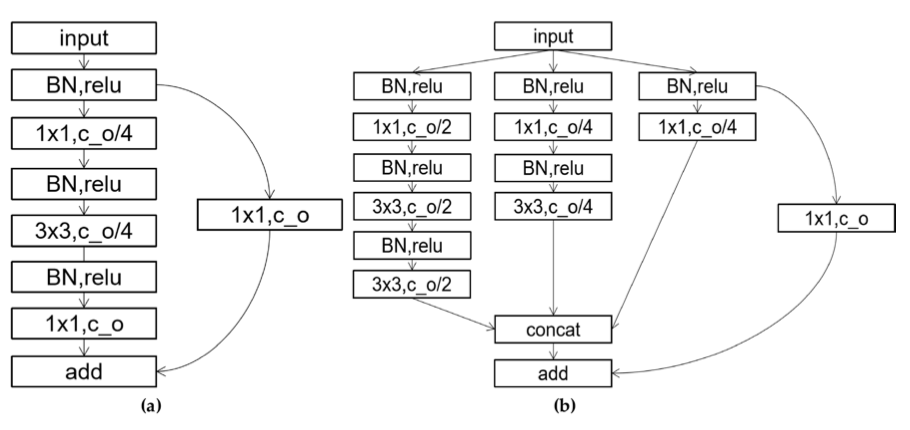
\includegraphics[width = 0.8\linewidth]{images/paper9/architecture.png}
    \centering
    \caption{(a) Structure of pre-activation residual unit (b) the large-size one}
    \label{fig:ResidualUnit}
\end{figure}

\subsubsection{Architecture}
The IE-CNN branch structure is the one shown in figure \ref{fig:IE-CNN ARCHITECTURE}. The local pathway 
is used to extract internal features and to improve fine-grained recognition 
performance. The global pathway instead captures the external features. 
The integration of all these features is carried out with a max-out merger 
strategy.
\begin{figure}[h!]
    \centering
    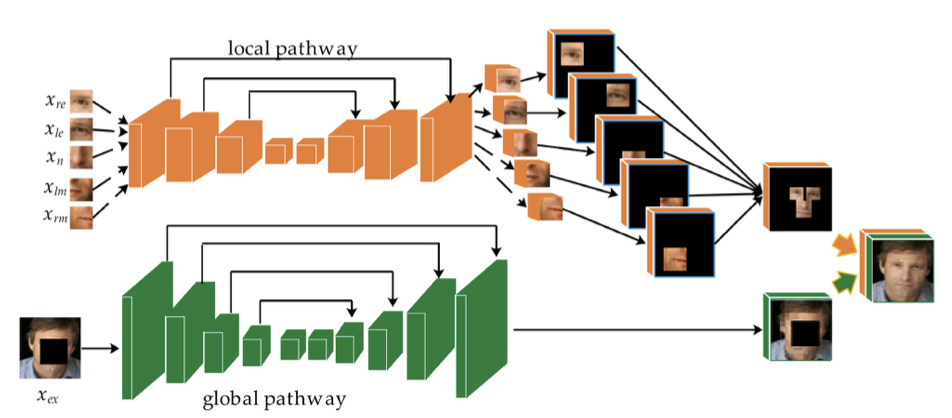
\includegraphics[width = 0.8\linewidth]{images/paper9/IE-CNN.png}
    \centering
    \caption{IE-CNN branch.}
    \label{fig:IE-CNN ARCHITECTURE}
\end{figure}

\subsubsection{Framework of the proposed training method}
The proposed model maps each image in a Euclidean space where, through 
the use of the distance L2, its similarity will be established. Following the 
\emph{LMNN} method \cite{0902694039}, three sets of images are created:
\begin{enumerate}
    \item $x^o$ (\emph{original}): represents the image of the face of a single individual;
    \item $x^p$ (\emph{positive}): represents the remaining images of the same individual;
    \item $x^n$ (\emph{positive}): represent the images of the faces of the other different 
    individuals.
\end{enumerate}
The aim is to have smaller Euclidean distances between $x^o$ and $x^p$. The 
input of the network consists of mini-batches, composed of images of positive 
and negative faces, composed of a few images useful for obtaining a better 
convergence during the descent of the stochastic gradient. In order to select 
the best set triples useful for training, the strategy to be used is to consider 
a $\theta$ margin in which the negative images $x^n$  will be found. Positive and 
negative image sets that have maximum distance will be chosen. 
\begin{figure}[h!]
    \centering
    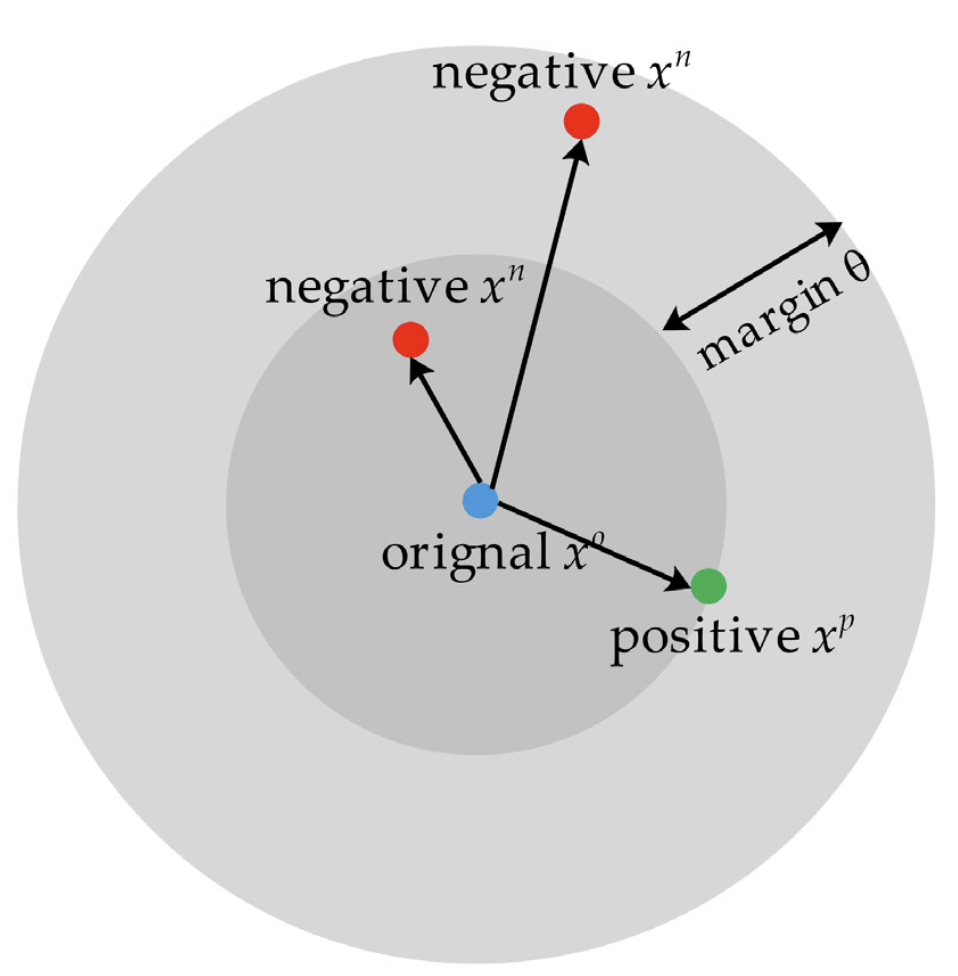
\includegraphics[width = 0.4\linewidth]{images/paper9/SET.png}
    \centering
    \caption{High-dimensional space.}
    \label{fig:HDS}
\end{figure}

The following are the steps performed on each original image $x^o$:
\begin{enumerate}
    \item Pre-processing: performed by a pre-trained CNN;
    \item Features enchancement: both external and internal;
    \item Mapping: in high-dimensional space.
\end{enumerate}

\subsection{EXPERIMENTAL RESULTS AND ANALYSIS}
\subsubsection{Experiment on feature map fusion in IE-CNN branch}
There are two methods for merging the outputs generated by the two pathways. 
The first, called $f_1$, performs a concatenation, while the second, called 
$f_2$, performs an element-wise sum. Table \ref{testAccuracyIE-CNN} shows the test accuracy, adopting 
the two merger strategies, on the two LFW and CASIA-WebFace datasets. 
As we can see, $f_1$ achieves the best score but on the other hand, due to the 
increase in parameters, this fusion method is time-consuming and requires a 
high computational cost.
\begin{table}[h!]
    \centering
    \begin{adjustbox}{max width=\textwidth}
    \begin{tabular}{|c|c|c|c|}
        \hline
        \bfseries{Fusion Strategy} & \bfseries{Operate Type} & \bfseries{LFW} &\bfseries{CASIA-WebFace}\\
        \hline
        $f_1$ & concatenate & \bfseries{96.23} & \bfseries{84.35}\\
        \hline
        $f_2$ & element-wise sum & 94.80 & 83.83\\
        \hline
    \end{tabular}
    \end{adjustbox}
    \caption{The test accuracy (\%) on LFW and CASIA-WebFace of IE-CNN branch with different fusion strategy.}
    \label{testAccuracyIE-CNN}
\end{table}

\subsubsection{Experimental Evaluation Index}
In order to evaluate the proposed method, two metrics are used: sensitivity 
(true positive rate) and accuracy. Another custom evaluation method used 
is that of \emph{Top1 \& Top5 precision}. In this metric $N$ represents the total 
number of images of a single individual, $N_1$ represents the number of images 
most similar (Grade1) while $N_5$ represent the least similar images (Grade5), 
therefore the precision is calculated as below:
\begin{equation}
    Precision_{top1}= \frac{N_1}{N}
\end{equation}
\begin{equation}
    Precision_{top5}= \frac{N_5}{N}
\end{equation}

\subsubsection{Experiments on LFW and CASIA-WebFace}
Another framework that has achieved good results in the field of similarity 
recognition is \emph{Inception-Resnet-v2} \cite{0902694022}. The performance of this method was 
compared with that of the proposed method. The triples used to train the 
models are identical (same original images, positive and negative). The number 
of images taken are divided into positive and negative. The accuracy and 
sensitivity achieved by both methods is visible in the image \ref{fig:compareV2}. Looking at 
the results, the accuracy and sensitivity achieved by the model are higher 
than those achieved by v1.
\begin{figure}[h!]
    \centering
    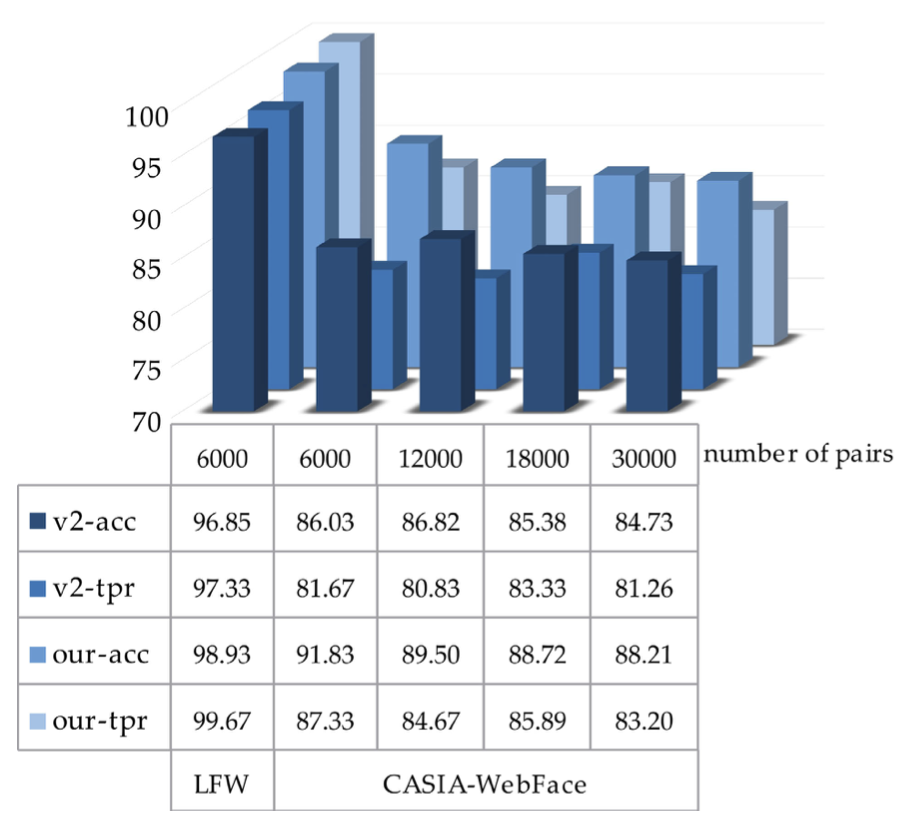
\includegraphics[width = 0.8\linewidth]{images/paper9/comparisonV2.png}
    \centering
    \caption{Comparison between v2 and the proposed methods on LFW and CASIA-WebFace datasets.}
    \label{fig:compareV2}
\end{figure}

\subsubsection{Top1\&Top5 Precision Experiments Under Different Global Scopes}
Comparisons were also made on the two personal Top1 \& Top5 precision 
metrics. The results obtained by both methods are those shown in table \ref{T12}.
\begin{table}[h!]
    \centering
    \begin{adjustbox}{max width=\textwidth}
    \begin{tabular}{|c|cc|cc|}
        \hline
        \multirow{2}{*}{Method} & \multicolumn{2}{c|}{LFW} & \multicolumn{2}{c|}{CASIA-WebFace}\\
        & Top5-acc & Top1-acc & Top5-acc & Top1-acc\\
        \hline
        v2 & 96.96 & 93.63 & 85.97 & 78.24\\
        \hline
        proposed & \bfseries{99.20} & \bfseries{98.86} & \bfseries{93.31} & \bfseries{84.92}\\
        \hline    
    \end{tabular}
    \end{adjustbox}
    \caption{Top1\&Top5 Precision (\%) between two methods.}
    \label{T12}
\end{table}

\subsubsection{Experiments On Similar Fase Dataset (SFD)}
In this experiment, the performance of another method called DeepID2+ \cite{0902694017} 
was also verified. The reference dataset in this case is just SFD. The experiment 
is conducted with images in which there are similar faces, divided by 
degrees. Also in this case accuracy and sensitivity are the metrics considered. 
In table \ref{SFDCompMeth} you can see the results obtained by all the models. As we 
can see, the lower the similarity level (towards grade 5), the higher the levels 
of accuracy and true positive rate achieved by the methods. The proposed 
method, however, managed to obtain the best performances also in this experiment. 
his Thighlights the importance of using external features that are 
not considered by the other methods.
\begin{table}[h!]
    \centering
    \begin{adjustbox}{max width=\textwidth}
    \begin{tabular}{|c|ccccc|}
        \hline
        \multirow{2}{*}{Method} & \multicolumn{5}{c|}{Similar Face Dataset (SFD)}\\
        & \RN{1} & \RN{2} & \RN{3} & \RN{4} & \RN{5}\\
        \hline
        DeepID2+ acc. & 49.73 & 59.75 & 58.64 & 64.37 & 66.33\\
        DeepID2+ tpr. & 71.77 & 78.08 & 76.28 & 81.77 & 83.17\\
        \hline
        v2 acc. & 42.81 & 54.75 & 55.64 & 66.97 & 68.22\\
        v2 tpr. & 63.33 & 70.00 & 65.33 & 71.67 & 68.08\\
        \hline
        proposed acc. & \bfseries{78.29} & \bfseries{83.19} & \bfseries{82.19} & \bfseries{86.11} & \bfseries{86.40}\\
        proposed tpr. & \bfseries{79.17} & \bfseries{83.33} & \bfseries{79.67} & \bfseries{85.67} & \bfseries{84.67}\\
        \hline
    \end{tabular}
    \end{adjustbox}
    \caption{Comparison abount v2, DeepID+ and proposd methods on SFD dataset}
    \label{SFDCompMeth}
\end{table}

\subsubsection{Supplementary Experiment on SFD}
The last experiment is carried out only between the v2 method, which does 
not use external features, and the one proposed. The aim is to see which of 
the two can best distinguish the similarities of faces. The values shown in the 
image \ref{fig:fei} represent the L2 distance between the upper and lower image. It can 
be seen that for v2, in all three images, the same face always appears, while 
the proposed method, thanks to the combination of external and internal 
features, manages to distinguish both people.
\begin{figure}[h!]
    \centering
    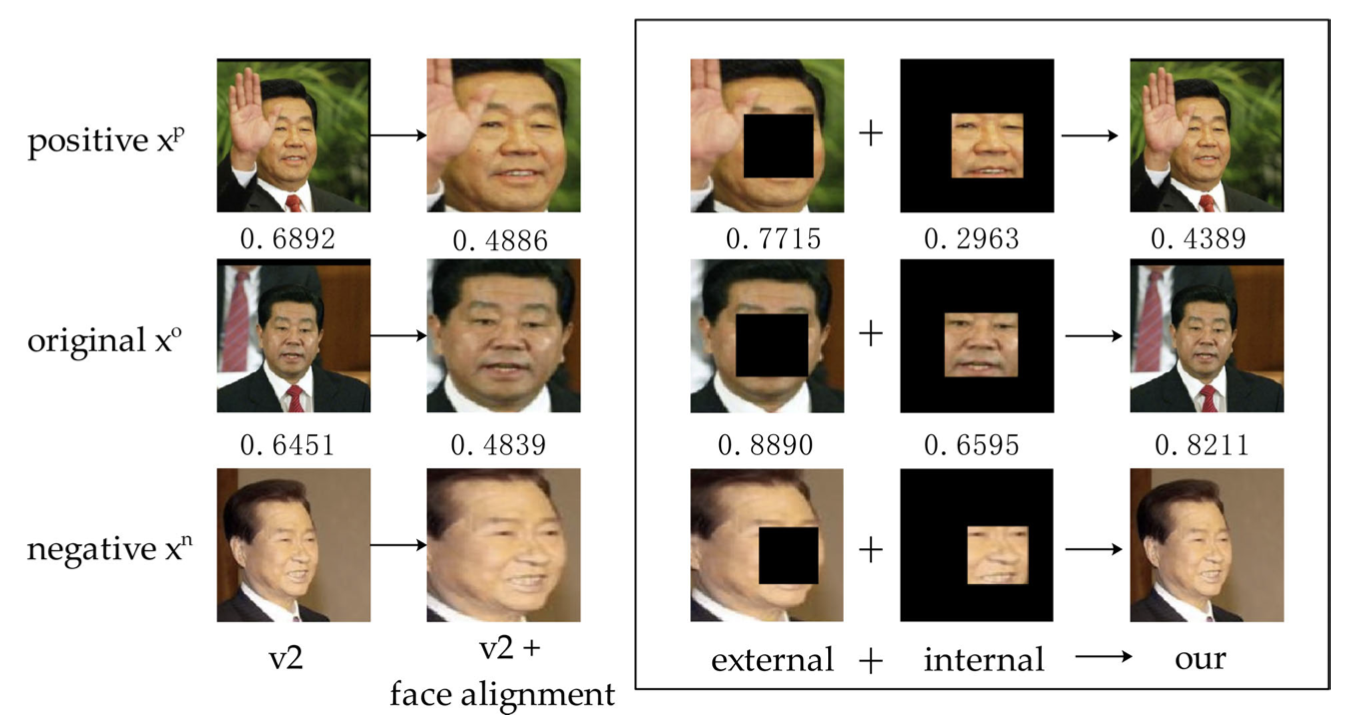
\includegraphics[width = 0.7\linewidth]{images/paper9/features.png}
    \centering
    \caption{The importance of external and internal features.}
    \label{fig:fei}
\end{figure}

\subsection{CONCLUSION}
What appears strange is that the greater the similarity between two faces, 
the lower the recognition accuracy achieved by all the models. Even if the 
addition of external and internal features represent a benefit for the purpose 
of recognition, at the computation level this operation turns out to be expensive 
in the training phase even if it is lightened by the use of mini-batches 
(triplet) and the various optimizations of the network.
